\section{Classification} \label{sec:BG:classification}
For a myoelectric prosthesis to be able to distinguish between movements it needs to perform, a control scheme is needed to categorize the movements. The control scheme is trained by being given information about the EMG signal represented as the features extracted from the raw EMG. If the features between each movement are well separated the control scheme is able to recognize each distinct movement. For this purpose classification control schemes are commonly used. A classifier categorizes each movement as a class, and based on the input features it gives one class as output at a time. Using a classifier thus limits the user to only performing movements which have been defined as classes. However, if trained properly a classifier can reach a low error rate for the trained movements \cite{Scheme2013}. A frequently used classification control scheme for myoelectric prosthetic control is the Linear Discriminant Analysis classifier (LDA) \cite{Englehart2003, Scheme2015, Fang2017, Scheme2013}. The advantage of LDA is that whilst having a low computation time it still enables robust control. An assumption about the LDA is that the input needs to be Gaussian distributed, which the EMG probability properties has shown to adhere to \cite{Duda2000, Nazarpour2013}. The following section provides further theoretical information about the LDA classifier.


\subsection{Linear Discriminant Analysis} \label{sub:BG:LDA}
LDA is a supervised classification method used to separate classes of data by linear decision boundaries. Each decision boundary is a hyperplane from which the shortest distance to each class feature value and class mean is maximized for each class. A decision boundary is defined as a linear combination of the feature values $x$ and is given as \cite{Duda2000}:

\begin{equation}
g(x) = w^tx +w_0
\end{equation}

where $w$ is a weight vector deciding the orientation of $g(x)$, and $w_0$ is a bias deciding the position of the hyperplane in relation to the origin. If $w_0 > 0$ the origin is on the positive side of the decision boundary, and if $w_0 < 0$ the origin is on the negative side. In the case of $w_0 = 0$ the decision boundary passes through origin. The distance from origin to the boundary is given as $\frac{w_0}{||w||}$. The position of the decision boundary is necessary to know to when separating features into regions. \cite{Duda2000}

In a two category case the decision rule for deciding classes is to decide class $w_1$ if $g(x) > 0$ and class $w_2$ if $g(x) < 0$. $g(x) = 0$ then defines the decision boundary that separates the features into two decision regions $R_1$ for $w_1$ and $R_2$ for $w_2$. The normal vector $w$ is orthogonal to any vector on the hyperplane, which is used to calculate the distance $r$ from feature values (x) to the decision boundary \cite{Duda2000}:

\begin{equation} \label{eq:featureValueDistance}
r = \frac{g(x)}{||w||}
\end{equation} 

The distance from origin and boundary to feature value (x) is needed to decide in which region the feature value belongs. \cite{Duda2000} These distances are illustrated in \figref{fig:geolda}.
%[[[[the distance from x to H is defining for the probability that x belongs to a region/class. The greater the distance to H the greater to possibility/likelihood that x is correclt classified to region 1 or 2]]]] 
%In \figref{fig:geolda} a geometric illustration of the linear discriminant function and its properties  is depicted.

\begin{figure}[H]                 
	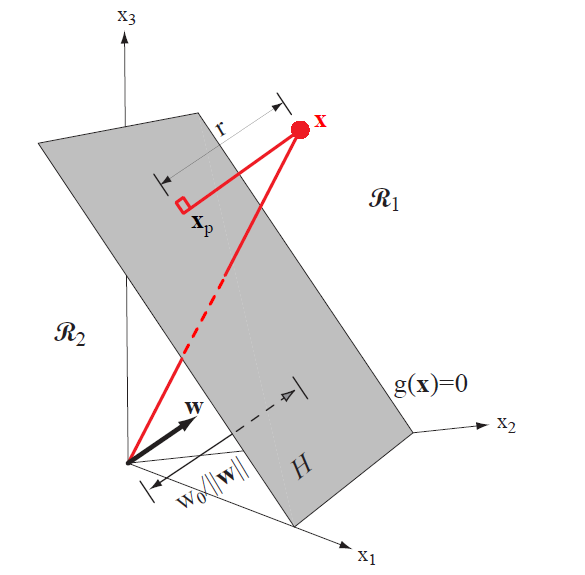
\includegraphics[width=.4\textwidth]{figures/xBackground/geolda}  
	\caption{A geometric illustration of the linear decision boundary $g(x)$ that separates the feature space into two decision regions $R_1$ and $R_2$. $x$ is the feature value, and $x_p$ is the point on the decision boundary in which $x$ is orthogonal projected on vector $w$. The distances from origin and boundary to feature value $x$ is marked red. \cite{Duda2000}}
	\label{fig:geolda} 
\end{figure}

When feature values are to be classified into more than two classes more decision boundaries are needed. This is a multicategory case in which $c$ numbers of boundaries are defined. When defining linear boundaries in this case any number can be chosen, but to minimize ambiguous decision regions the boundaries are defined by \cite{Duda2000}:

\begin{equation} \label{eq:multicase}
g_{i}(x) = w^tx_{i} +w_{i0} ~~~~~~~~~~~ i = 1,...,c,
\end{equation}

This equation follows the notation of the two-category case, with the addition of $i$ numbers of boundaries, feature values and biases. This type of classifier is called a linear machine, dividing the feature space into $c$ regions. A liner machine will be adopted as classification method in this project. Regions $R_i$ and $R_j$, that are connected is divided by a boundary hyperplane $H_{ij}$ defined by \cite{Duda2000}:

\begin{equation}
g_i(x) = g_j(x)
\end{equation}

Often regions are contiguous and will have a single boundary to separate several regions. \cite{Duda2000} Illustrations of this case can be seen on \figref{fig:LMregions}. 

\begin{figure}[H]                 
	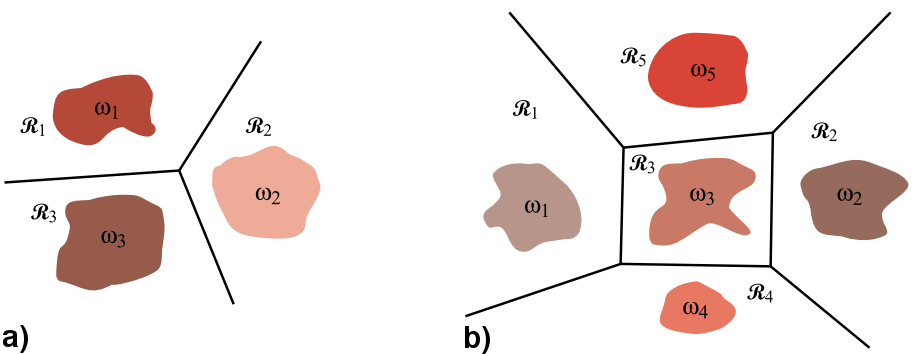
\includegraphics[width=.6\textwidth]{figures/xBackground/LMregions}  
	\caption{A three class $(a)$ and five class $(b)$ case each respectively separated by one decision boundary linear machine. \cite{Duda2000}}
	\label{fig:LMregions} 
\end{figure}

When the decision boundaries $g_i(w)$ have been calculated as in \eqref{eq:multicase}, the input feature values can be decided upon which class they belong to by calculating the distance to the decision boundary as in \eqref{eq:featureValueDistance}. 


%\subsection{Gradient descend/minimum criterion function}


\subsection{Classification confidence scores} \label{sub:BG:classificationConfidenceScores}
An additional reason for using LDA as control scheme is because it enables the calculation of confidence scores for the classes, which will be used in the user training described in \secref{sec:BG:userTraining} to improve the prosthesis control. Based on the classification of feature values by the linear machine, confidence scores for the classes can be evaluated by computing the posterior probability of each class. Calculating the posterior probability is possible by knowing the likelihood $P(x|w_j)$ and the prior probability $P(w)$.
%The likelihood is the conditional probability the feature value $x$ can appear in a certain class ($w_j$), while the prior probability $P(x)$, is the probability of a feature value appearing. %is this not always 100% in our case?
The posterior probability for a class is a value between 0 and 1, and is calculated as follows:

\begin{equation}
P(w_j|x) = \frac{P(x|w_j)P(w)}{P(x)}
\end{equation}

where $w_j$ represents a class and x represents a feature value. The posterior probability is given as the product of the class conditional probability, $P(x|w_j)$ and the prior probability $P(w)$ divided by a normalization term $P(x)$ that guaranties that the posterior probabilities for all classes sums to one. $P(x|w_j)$ is the probability of obtaining a feature value when selecting samples randomly from a class. $P(w)$ is the probability of a sample from a specific class appears in its correct class, before it have actually appeared. Summation of posterior probabilities for all classes will equal 1.
